\chapter{显著区域检测在图像检索上的应用}

\section{引言}
显著区域检测作为一项预处理基础,其算法的有效性必须要结合相应的应用才能进行准确的评估。在目前国际的主流研究工作中,对显著区域检测的评估都是基于其在图像分割中的表现。然而,到目前为止,还没有针对显著区域检测在其它应用领域(如图像检索、目标检测等)的研究和评估工作。在本章中,我们选取了图像检索这个领域,评估了我们的显著区域检测算法在图像检索中的有效性。在下面的文章中,我们将首先对基于内容的图像检索进行简单的介绍,着重介绍了基于词袋模型的图像检索系统。随后,我们将显著区域检测算法应用于图像检索系统中,实验分析、评估了显著区域检测在图像检索中的作用。

\section{基于内容的图像检索系统}

\subsection{图像检索简介}
基于内容的图像检索(Content-based image retrieval)是在给定查询图像的前提下,依据内容信息或指定查询标准,在图像数据库中搜索并找出符合查询条件的相应图片\cite{cyy2007img}。

随着网络以及多媒体技术的迅速发展,数字图像的数量正在不断迅速的增长,对数字图像的自动化管理与检索,也成为新时代迫切的需求。然而,传统的基于关键字检索的方式,需要人工对图像内容进行标注,不仅工作量巨大,同时也存在人工标注的文字歧义等问题。在这样的背景下,基于内容的图像检索技术应运而生。

最早的基于内容的图像检索应用成功的是IBM开发的QBIC\cite{qbic}(Query By Image Content)系统,通过用户指定按例子查询或者按绘制草图查询,它利用了颜色、纹理、形状等特征对图像进行分析,从而查找出符合用户意图的图像。

由于基于内容的图像检索技术从图像内容本身出发,无需人工干预或者主动标记,大大减轻了多媒体管理人员的负担,因而被广泛的应用于电子图书馆、医学分析、博物馆等领域;与此同时,基于内容的图像检索也常常用于网购、拷贝检测等大众产品之中。

基于内容的图像检索通常对整幅图像进行分析,提取特征,然后在数据库中查找相似图像。然而,用户的查询意图常常并非充斥于整幅图像之中。对整幅图像进行特征提取的同时,也会将非用户意图部分(如图像背景)计算在内,从而影响最终的查询结果与精度。

显著区域检测则恰好可以解决这个问题,通过显著区域检测标记出用户感兴趣的区域,仅仅在用户感兴趣的区域提取特征并检索,能减少用户意图鸿沟,提高检索效率与效果。

在本章的接下来的部分,我们将首先介绍经典的BOW模型,并根据此模型实现一个图像检索系统。接下来,我们将显著区域检测与该系统相结合,最后,我们通过实验验证效果,以原系统为baseline,对比现系统添加显著区域检测后的提升。

\subsection{基于词袋模型的图像检索系统}
在大规模图像检索系统中,词袋模型(BOF)是目前为止最为成功的模型之一\cite{arandjelovic2012three},相比其它模型(如VLAD\cite{arandjelovic2013all}, FisherVector\cite{perronnin2010large}),BOF具有易于实现,扩展众多的优点,非常利于工程化实现调优。

\begin{figure}
\centering
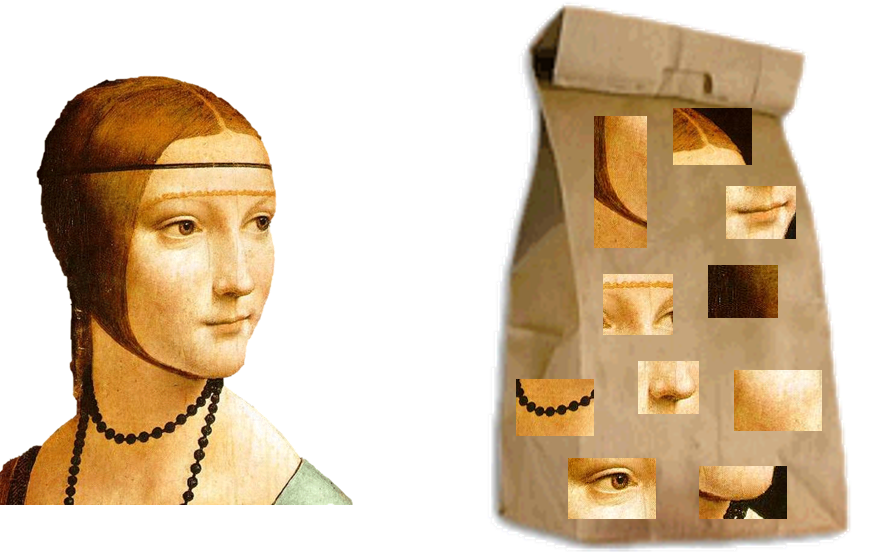
\includegraphics[width=0.7\textwidth]{bow.png}
\caption{BOW模型}
\end{figure}

词袋模型在图像上提取局部特征点,并通过kmeans等方法将特征向量聚类,形成视觉单词的码书。在线检索时,通过将提取到的局部特征点映射为视觉单词,则可以将整个图像看做是由视觉单词组成的文本,从而可以应用文本检索的经典方法来对图像进行检索。下面我们将对基于BOF模型的图像检索系统进行简单的介绍。


\subsubsection{SIFT特征提取}
SIFT,即尺度不变性特征(Scale-invariant feature transform, SIFT),是图像处理与计算机视觉领域广泛使用的一种局部特征描述子\cite{lowe2004distinctive}。其具有以下一些特性:
\begin{enumerate}
\item SIFT特征是图像的局部特征,对旋转、尺度缩放、亮度变化等均具有不变形,对视角变化、仿射变换、噪声也具有一定程度的稳定性;
\item 独特性好,信息量丰富,适于在海量特征数据库中进行快速、准确的匹配;
\item 多量性,即使少数的几个物体也可以产生大量的SIFT特征向量;
\item 高速型,经优化的SIFT匹配算法甚至可以达到实时的要求;
\item 可扩展性,可以很方便的与其他形式的特征向量进行联合;
\end{enumerate}
正是因为SIFT具有以上特性,BOF模型通常都选用SIFT对图像局部特征进行描述。SIFT特征检测主要包括以下4个基本步骤:
\begin{enumerate}
\item 尺度空间极值检测:搜索所有尺度上的图像位置,通过高斯微分函数来识别潜在的对于尺度和旋转具有不变性的兴趣点。
\item 关键点定位:在每个候选位置上,通过一个拟合精细的模型来确定位置和尺度,依据候选点的稳定程度选取关键点。
\item 方向确定: 基于图像局部的梯度方向,分配给每个关键点位置一个或多个方向,后面对关键点的特征描述都相对于关键点的方向,尺度和位置进行变化,从而保证特征描述的不变性。
\item 关键点描述:在每个关键点周围的领域内,根据所选尺度,在图像局部计算梯度直方图,并连接为一个128维的向量。
\end{enumerate}

\subsubsection{建立码书}
对于每个图像,提取得到若干SIFT特征点向量,然后对所有图像的特征向量进行聚类,通常使用k-means聚类,最后将聚类得到的聚类中心作为视觉单词,形成码书。假设要形成k个视觉单词,k-means算法描述如下:
\begin{enumerate}
\item 适当选择k个类的初始中心;
\item 在第i次迭代中,对任意一个样本,求其到k个中心的距离,将该样本归到距离最短的中心所在的类;
\item 利用均值等方法更新该类的中心值;
\item 对于所有的k个聚类中心,如果重复利用2,3步骤进行迭代更新后,值保持不变(或者指定一个变化阈值),则迭代结束,否则继续迭代。
\end{enumerate}

在实际操作中,通常在另外一个数据集上提取特征并建立码书,视觉单词数量k通常选取20k至200k之间。

\subsubsection{倒排索引}
在线实际检索时,由于通常图像库很大(例如百万级别),此时如果通过线性比较计算图像之间的相似性,速度是不可忍受的,为此需要建立某种形式的索引,以提高检索效率。通常采用倒排索引。
\begin{figure}[h]
\centering
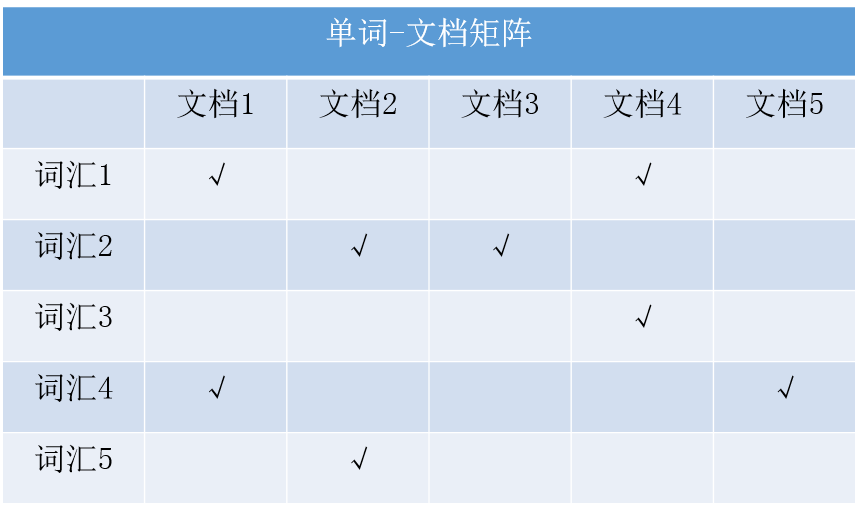
\includegraphics[width=0.8\textwidth]{invindex.png}
\caption{倒排索引示例}\label{fig:invindex}
\end{figure}
如图\ref{fig:invindex}所示为一个单词-文档矩阵,其中打勾则代表包含关系。从纵向即文档的维度来看,每列代表文档包含了哪些单词,即正向索引。而横向即从单词的维度来看,每行代表了哪些文档包含了某个单词。倒排索引即从单词的维度来看,建立的单词-文档矩阵。如此建立索引后,每次在线查询时,只需要将得到的局部特征映射为视觉单词,然后通过倒排索引的单词-文档矩阵,就可以查找到所有包含该单词的文档,最后通过tf-idf进行评分,即可将相关的文档进行评分。倒排索引高效的关键在于,每个文档包含的视觉单词只是整个码书很小的一部分,即单词-文档矩阵是稀疏的,这样在检索时,只需要计算码书中非0部分的评分,从而避免了在整个码书上计算。

\subsection{整体系统框架}
\begin{figure}[h]
\centering
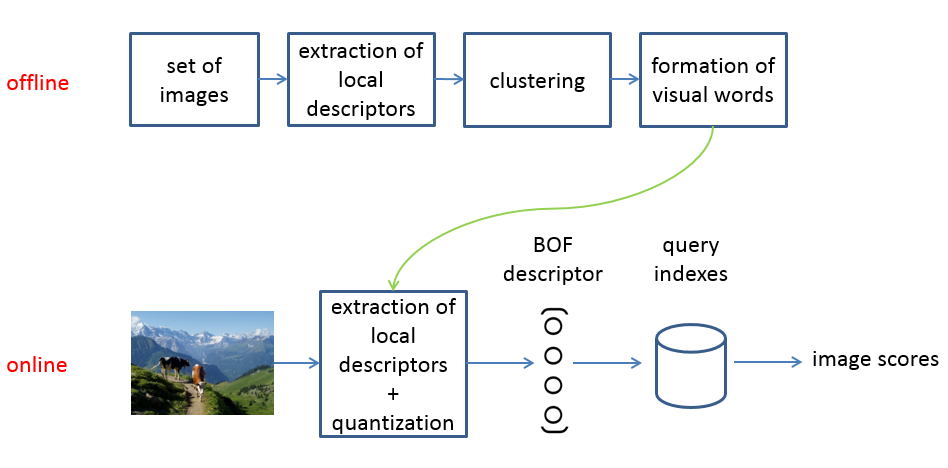
\includegraphics[width=\textwidth]{bowframework.png}
\caption{BOW模型框架图}\label{fig:bowframework}
\end{figure}
整体框架如图\ref{fig:bowframework}所示,离线训练时,我们从一组图像集合中提取局部特征,然后对其进行k-means聚类,我们将聚类中心作为视觉单词,形成码书。在线检索时,我们首先提取图像的局部点特征(SIFT),然后将每一个点特征进行量化(查找与码书中的视觉单词欧氏距离最近的单词),形成词频向量,最后通过倒排索引,对相关图像进行评分,排序后,输出相关文档(图像)。

\section{利用显著区域检测优化结果}
\subsection{问题描述}
\begin{figure}[h]
\centering
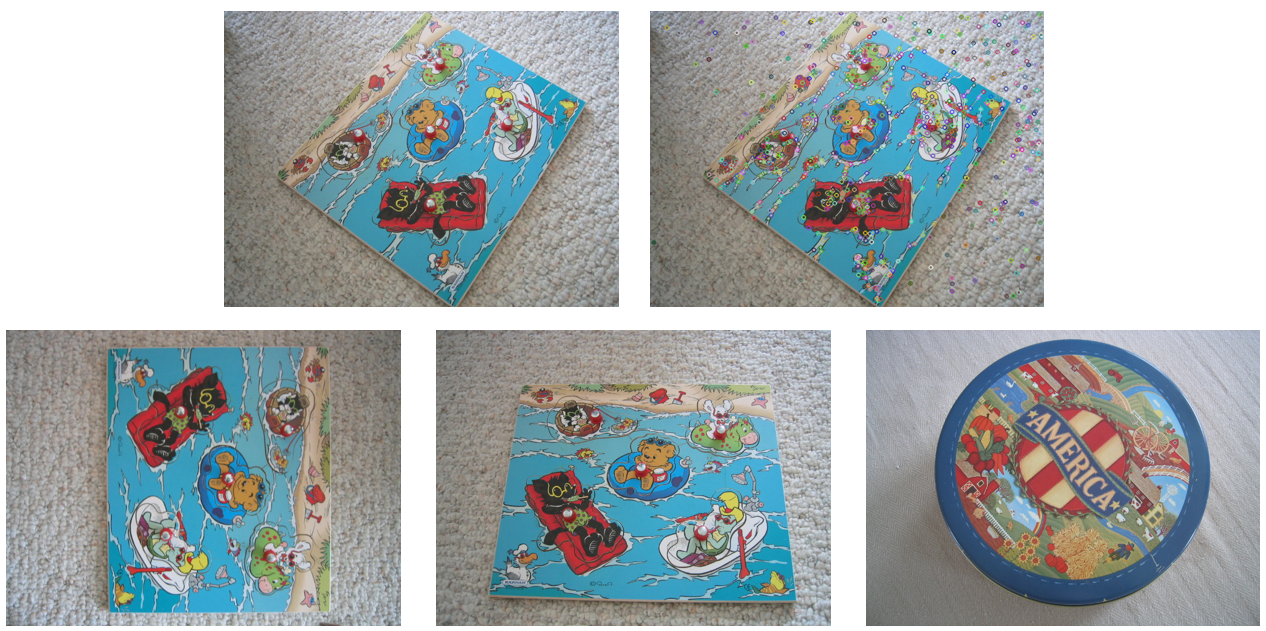
\includegraphics[width=\textwidth]{problem.png}
\caption{检索示例}\label{fig:problem}
\end{figure}

如图\ref{fig:problem}所示,第一行左边的图像为输入图像,第二行为检索结果的前三幅图像(除去该图像自身),可以看到第三幅图像是错误的。我们可视化了在输入图像上检测到的SIFT特征点(第一行右边的图像),可以看到,由于该图像的背景区域是凹凸不平的地毯材料,存在很多类blob型的斑点,故在该图像的背景上也提取到了很多SIFT点。然而这些SIFT点并非对我们需要检索的主体对象的描述,而且区分性不高,故背景上大量检测到的这些SIFT对检索结果产生了影响,致使检索精度降低。

从这个例子我们可以看到,背景元素通常与用户的检索意图无关,然而背景元素上提取到的特征点,却同样参与了图像相关性的评分,因而会影响到图像检索系统的精度。

\subsection{优化方案}
针对上述误匹配问题,研究者们也提出了各种各样的方案:
\begin{enumerate}
\item RANSAC。图像配准中常用,通过随机抽样一致性,排除误匹配的点,计算复杂度高。
\item 停用词列表(Stop List)\cite{sivic2003video}。如果一个视觉单词在几乎大部分图像中都出现了,那么这样的视觉单词是缺乏分辨力的,应该被抑制。
\item 海明空间嵌入(HE)\cite{jegou2008hamming}。适用于由于码书太小造成的局部特征向量量化精度不足。
\item 弱几何空间关系校验(WGC)\cite{jegou2010improving}。两幅匹配的图像,其匹配点应该具有尺度一致性和主方向一致性,通过这样的几何空间关系的校验,能够过滤许多误匹配点。
\end{enumerate}

然而这些方法都有各自的一些不足,例如,停用词列表的选择常常具有经验性(停用词选择过多,会降低视觉单词的匹配率,选择过少,又无法起到过滤作用),需要进行多次尝试;使用几何空间关系校验可以很好的处理误匹配问题,但是由于需要在索引中加入几何空间信息,所以内存占用会大大增加。

在我们的方案中,我们采用显著区域检测做预处理,将前景和背景分离出来,提取特征点的时候,只在显著区域计算特征点,而忽略背景区域的特征点。我们的方法具有如下三个优势:
\begin{enumerate}
\item 检索结果更加准确。剔除了背景上的特征点后,能在一定程度上减少误匹配,使得检索结果更加准确,同时更加符合用户意图。
\item 检索速度略有提升。首先特征提取只需在显著区域进行计算,特征提取时间有所降低;其次,过滤掉背景上的局部特征点后,需要在倒排索引上检索的次数也大大减少了。
\item 我们的方案可以与现有系统完美集成,只需略微修改特征提取的代码,无需重新生成索引,也不会增加内存的占用。
\end{enumerate}

在实验中,我们选取了前一章中介绍的基于蒙特卡洛采样的显著区域检测算法。同时,我们只在在线检索的时候应用我们的算法对待检索图像进行处理,图像入库建立索引的时候仍然计算全图像的局部特征。

\section{实验结果}
\subsection{数据集和评价指标}
我们使用了ukbench数据集\cite{nister2006scalable},这个数据集包含2550种不同的物体或场景,每一个物体(场景)都包含4幅从不同角度拍摄的图像,整个数据集一共有10200幅图像。对于这个数据集,我们采用两种评价指标:mAp(mean Average Precision)和KS(Kentucky Score),KS指标是该数据集的作者针对该数据集提出的评价指标,即取top 4的结果中,正确结果的平均值。另外,为了更加客观的比较优化方案的优化效果,我们分别取码书大小为20k和200k的结果做比较。

\subsection{实验结果}
\begin{table}[h]
\centering
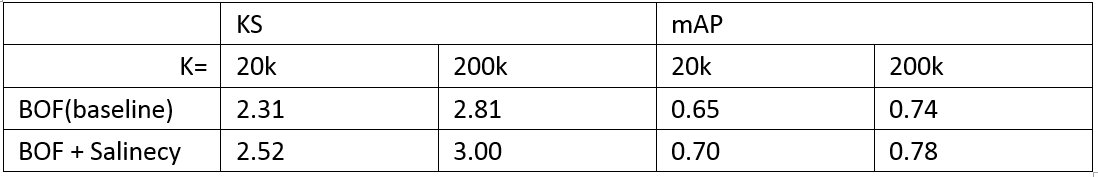
\includegraphics[width=\textwidth]{exp.png}
\caption{实验结果}\label{tab:sal_res}
\end{table}

我们采用最原始的BOF模型作为我们的baseline, 同时选取了码书大小为分别为20k和200k时的结果进行比较。实验结果如表\ref{tab:sal_res}所示,可以看到,码书大小为200k的情况下,检索的精度明显有所提高,这是由于更加密集的聚类中心使得量化误差更小,视觉单词的区分度更高。另外,在添加了显著区域检测进行特征点的过滤后,无论是k=20k还是200k的情况下,检索性能均有所提升,KS值普遍提高了0.2左右,同时mAp提高了4个百分点左右,实验证明,显著区域检测对图像检索的性能确实有一定的提升作用。同时,我们在图\ref{fig:sal_res}中也列出了一些我们的检索结果实例,其中红线左侧为待检索图像,右侧列出了检索结果的前三。可以看到,我们的系统虽然仅仅基于基础的BOF系统+显著区域检测,但是仍然具有良好的准确率,并能应对一定程度的视角和旋转变换。

\begin{figure}[h]
\centering
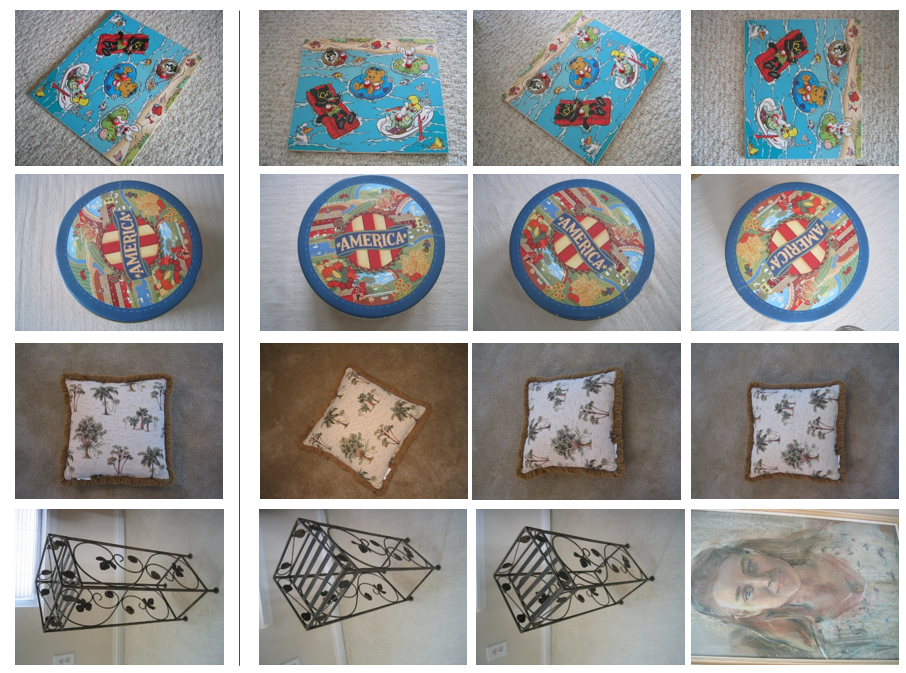
\includegraphics[width=\textwidth]{sal_res.png}
\caption{检索效果示例}\label{fig:sal_res}
\end{figure}
